\documentclass[10pt]{beamer}
\usetheme[progressbar=frametitle]{metropolis}

\usepackage{appendixnumberbeamer}

\usepackage{slashed}
\usepackage{booktabs}
\usepackage[scale=2]{ccicons}
\usepackage{braket}
\usepackage{pgfplots}
\usepgfplotslibrary{dateplot}
\usepackage{xspace}
\usepackage{dsfont}
\usepackage{fontspec}
\usefonttheme[onlymath]{serif}

\newcommand{\husk}[1]{\color{red} #1 \color{black}}
\newcommand{\themename}{\textbf{\textsc{metropolis}}\xspace}
\newcommand{\D}{\mathcal{D}}
\DeclareMathOperator{\Tr}{tr}								% For matrix traces
\DeclareMathOperator{\tr}{tr}								% For matrix traces

\title{Lattice Quantum Chromo Dynamics}
% \subtitle{\textit{Kvantefargedans på et gitter}}
\date{\today}
\author{Giovanni Pedervia, Mathias Vege}
\institute{University of Oslo}

\begin{document}

\setbeamercolor{background canvas}{bg=white}
\maketitle

% \begin{frame}{Overview}
%   \setbeamertemplate{section in toc}[sections numbered]
%   \tableofcontents[hideallsubsections]
% \end{frame}

%%%%%%%%%%%%%%%%%%%%%%%%%%%%%%%%%%%%%%%%%%%%%%%%%%%%%%%%%%%%%%%%%%%%%%%%%%%%%%%%%%%%%%%%%%
\section{Introduction}
%%%%%%%%%%%%%%%%%%%%%%%%%%%%%%%%%%%%%%%%%%%%%%%%%%%%%%%%%%%%%%%%%%%%%%%%%%%%%%%%%%%%%%%%%%

\begin{frame}{The fundamental forces}
	There are four fundamental forces in nature
	\begin{itemize}
		\item Gravity
		\item Electromagnetism
		\item Weak force
		\item Strong force
	\end{itemize}
\end{frame}

\begin{frame}{Coupling of the forces}
	Hope that at some energy these couplings will be equal.
	\husk{picture of couplings here}
\end{frame}

\begin{frame}{The Standard Model}
	\begin{align}
		\mathcal{L} &= - \frac{1}{4}(F_{\mu\nu})^2 + i\bar{\psi}\slashed{D}\psi + h.c. \\
		&+ \bar{\psi}_i y_{ij}\psi_j \phi + h.c. + |D_\mu\phi|^2 - V(\phi)
	\end{align}
	But we are only interested in the strong force...
\end{frame}

\begin{frame}{QCD}
	The full QCD Lagrangian,
	\begin{align}
		\mathcal{L} = -\frac{1}{4} G_{\mu\nu}^a {G^{\mu\nu}}^a + \bar{\psi}_i (i\gamma^{\mu} D_{\mu}_{ij} - m\delta_{ij})\psi_j
	\end{align}
	$a$ is color indices, $i,j$ is flavour indices. $D_\mu = \partial_\mu - i g t^a A_\mu^a$.
\end{frame}

\begin{frame}{Why QCD is weird}
	\begin{itemize}
		\item In the low energy limit, QCD is non-perturbative!
		\item Self-interaction
	\end{itemize}
\end{frame}

%%%%%%%%%%%%%%%%%%%%%%%%%%%%%%%%%%%%%%%%%%%%%%%%%%%%%%%%%%%%%%%%%%%%%%%%%%%%%%%%%%%%%%%%%%
\section{Lattice QCD}
%%%%%%%%%%%%%%%%%%%%%%%%%%%%%%%%%%%%%%%%%%%%%%%%%%%%%%%%%%%%%%%%%%%%%%%%%%%%%%%%%%%%%%%%%%

\begin{frame}{Solution: Lattice QCD}
	\begin{itemize}%[<+->]
		% \item Why Lattice QCD? Or QCD in general?
		\item Low-energy regime is non-perturbative.
		\item To understand nuclear forces, one needs a first principles approach.
		\item Understanding nuclear physics from LQCD.
		\item Can be used to investigate Dark Matter phenomena.
	\end{itemize}
\end{frame}

\begin{frame}{Challenges with LQCD}
	\begin{itemize}%[<+->]
		\item Create a program that...
		\begin{itemize}%[<+->]
			\item generates field configurations.
			\item flows generated field configurations.
			\item Samples the field for $P$, $E$, $Q$, $Q_{t_e}$.
		\end{itemize}
		\item Take care of technicalities such as parallelization, $SU(3)$ exponentiation, ect.
		\item Perform analysis with bootstrap, jackknife, autocorrelation.
		\item Side projects: animating the field energy density and topological charge.
	\end{itemize}
\end{frame}

\begin{frame}{Lattice QCD}
	\begin{itemize}%[<+->]
		\item Requirement of \textit{Gauge invariance} is strongly maintained(throws Lorentz invariance out of the window ect.).
		$U' = \Omega^\dagger(x) U \Omega(x)$
		\item Discretizing the Gluon field in spacetime by introducing \textit{link variables}, $U_\mu(x)$.
	\end{itemize}
\end{frame}

\begin{frame}{Path integrals}
	For field theories we discretize the field into points in space time. For a scalar field, this becomes 
	\[
		 \int \D \phi \rightarrow \int \prod_{x_i \in lattice} d\phi(x_i)
	\]
	From this we can extract observables $\Gamma[\phi]$ dependent on this field as
	\[
		\braket{\Gamma[\phi]} = \frac{1}{Z} \int \D \phi \Gamma[\phi] e^{-S[\phi]}
	\]
	where the normalization $Z$ is given again by 
	\[
		Z = \int \D \phi e^{-S[\phi]}
	\]
\end{frame}

%%%%%%%%%%%%%%%%%%%%%%%%%%%%%%%%%%%%%%%%%%%%%%%%%%%%%%%%%%%%%%%%%%%%%%%%%%%%%%%%%%%%%%%%%%
\section{Fun technicalities}
%%%%%%%%%%%%%%%%%%%%%%%%%%%%%%%%%%%%%%%%%%%%%%%%%%%%%%%%%%%%%%%%%%%%%%%%%%%%%%%%%%%%%%%%%%

\begin{frame}{Parallelization}
	\begin{itemize}%[<+->]
		\item How do you share a face in 4D?
		\item 3 different approaches
		\begin{itemize}%[<+->]
			\item \textbf{Face-sharing}. Edge cases, not possible in the Metropolis algorithm
			\item \textbf{Single link-sharing}. Relatively simple to implement, but slow if network is slow.
			\item \textbf{Shifts}. Large non-blocking data packets at a time.
		\end{itemize}
		% \item Example on 
		% \begin{align}
		% 	U_{\mu\nu} &= U_\mu(n)U_\nu(n+\hat{\mu})U_\mu(n+\hat{\nu})^\dagger U_\nu(n)^\dagger
		% \end{align}
	\end{itemize}
\end{frame}

\begin{frame}{Sampling}
	Data is generated with the Metropolis algorithm, and following setup,
	\begin{itemize}
		\item Thermalize lattice. Roughly $~10000$ updates.
		\begin{enumerate}
			\item Perform $N_{corr}$ updates on the \textit{whole} Lattice.
			\item For each $N_{corr}$ update, we also perform $N_{up}$ updates on every \textit{single} link.
			\item Measure the change in $\Delta S$, the action at each update. Accept config if $\exp(-\Delta S) > r$, where $r$ is a number drawn from a uniform distribution.
			\item Flow the lattice and calculate observable at each step or save it to file.
		\end{enumerate}
	\end{itemize}
\end{frame}

\begin{frame}{Flow}
	\textit{A way of renormalizing the field.}
	% \begin{figure} % Illustrate with animation
	% 	\includegraphics[width=0.6\textwidth]{figures/correlator_smearing.gif}
	% 	\caption{Smearing of a correlator, $\langle Q_{t_e} Q_{t_{e,0}} \rangle$}
	% \end{figure}
\end{frame}

\begin{frame}{Data}
	\begin{table}
		\caption{Every set is generated with 600 correlation updates between each configuration, and 30 updates per link, except for $6.45$, which has 1600 correlation updates. The the side of the cube is then around $L=2.2$ fermi.}
		\begin{tabular}{l | l | l | l}
			$\beta$ & Size & $N_{cfgs}$ & Size \\ \hline
			$6.0$ & $24^\times 48$ & $1000$ & 356 GB \\
			$6.1$ & $28^\times 56$ & $500$ & 330 GB\\
			$6.2$ & $32^\times 64$ & $500$ & 562 GB\\
			$6.45$ & $48^\times 96$ & $250$ & 1.4 TB\\
		\end{tabular}
		\label{tab:data_batches}
	\end{table}
\end{frame}

%%%%%%%%%%%%%%%%%%%%%%%%%%%%%%%%%%%%%%%%%%%%%%%%%%%%%%%%%%%%%%%%%%%%%%%%%%%%%%%%%%%%%%%%%%
\section{Observables}
%%%%%%%%%%%%%%%%%%%%%%%%%%%%%%%%%%%%%%%%%%%%%%%%%%%%%%%%%%%%%%%%%%%%%%%%%%%%%%%%%%%%%%%%%%

\begin{frame}{Plaquette}
	The \textit{plaquette} is the simplest possible gauge invariant object on the lattice. It is a square made of 4 link variables:
	\begin{align}
		P_{\mu\nu} &= U_\mu(n)U_\nu(n+\hat{\mu})U_{-\mu}(n+\hat{\mu}+\hat{\nu})U_{-\nu}(n+\hat{\nu}) 
		&= U_\mu(n)U_\nu(n+\hat{\mu})U_{\mu}(n+\hat{\nu})^\dagger U_{\nu}(n)^\dagger
	\end{align}
	\begin{center}
		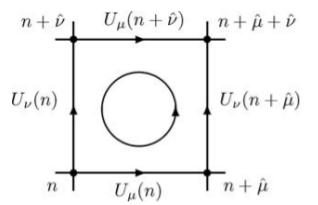
\includegraphics[scale=0.4]{figures/plaq.png}
	\end{center}
\end{frame}

\begin{frame}{Energy}
	\begin{align}
		\langle E\rangle = -\frac{1}{64V}F_{\mu\nu}^a{F^a}^{\mu\nu}
	\end{align}
\end{frame}

\begin{frame}{Tological charge}
	Can be thought of as the curl of the gluon field. Analogous to $u \times v = \varepsilon^{ijk} u_j v_k$
	\begin{align}
		Q = - \sum_x \frac{1}{64 \cdot 32\pi^2}\epsilon_{\mu\nu\rho\sigma}Tr\{G^{clov}_{\mu\nu}G^{clov}_{\rho\sigma}\}
	\end{align}
\end{frame}

\begin{frame}{Topological Susceptibility}
	\begin{align}
		\chi^{1/4} = \frac{\hbar c}{aV^{1/4}}\langle Q^2 \rangle^{1/4}
	\end{align}
\end{frame}

\begin{frame}{$N_f$ - checking the flavor}
	% Using Witten-Veneziano formula\footnote{See article following for an example of using WV: https://arxiv.org/pdf/hep-th/0407052.pdf} to look at how different $\chi$ behave in the continuum limit and which that gives the best error estimate.
	Using Witten-Veneziano formula to look at how different $\chi$ behave in the continuum limit and which that gives the best error estimate.
	\begin{align*}
		\frac{F_\pi^2 m_{\eta'}^2}{2 N_f} = \chi
	\end{align*}
	where $F_\pi$ is the decay rate constant of pion given as $F_\pi=130.0\pm5.0$MeV. The mass of the meson $\eta'$ is given as $m_{\eta'}=957.78\pm0.06$MeV. $N_f$ is the number of flavors.
\end{frame}


% %%%%%%%%%%%%%%%%%%%%%%%%%%%%%%%%%%%%%%%%%%%%%%%%%%%%%%%%%%%%%%%%%%%%%%%%%%%%%%%%%%%%%%%%%%
% \section{The Effective Mass}
% %%%%%%%%%%%%%%%%%%%%%%%%%%%%%%%%%%%%%%%%%%%%%%%%%%%%%%%%%%%%%%%%%%%%%%%%%%%%%%%%%%%%%%%%%%
% \begin{frame}{Investigating the $\langle Q_{t_e} Q_{t_e=0} \rangle$}
% 	\begin{figure}
% 		\includegraphics[width=0.9\textwidth]{../../../LatticeAnalyser/figures/data8/post_analysis/qtq0e/betaall_N0123/post_analysis_qtq0e_bootstrap_te000.png}
% 		\caption{$\langle Q_{t_e} Q_{t_e=0} \rangle$ taken at four flow times, $t_f = 0, 50, 200, 400$.}
% 		% \caption{t}
% 	\end{figure}
% \end{frame}

% \begin{frame}{Investigating the $\langle Q_{t_e} Q_{t_e=0} \rangle$}
% 	\begin{figure}
% 		\includegraphics[width=0.9\textwidth]{../../../LatticeAnalyser/figures/data8/post_analysis/qtq0e/slices/te0.00/post_analysis_qtq0e_bootstrap_tf999.png}
% 		\caption{$\langle Q_{t_e} Q_{t_e=0} \rangle$ taken at flow time $t_f = 999$.}
% 	\end{figure}
% \end{frame}

% \begin{frame}{Investigating the $m_{eff}$}
% 	Effective mass of the topological instantons given at $\beta = 6.2$
% 	\begin{align}
% 		m_{\text{eff}} = a \ln \left( \frac{\langle Q_{t_e} Q_{0} \rangle}{\langle Q_{t_e + 1} Q_{0} \rangle} \right)
% 	\end{align}
% 	\begin{figure}
% 		\includegraphics[width=0.7\textwidth]{../../../LatticeAnalyser/figures/data8/beta62/qtq0eff/tflow0999/qtq0eff_bootstrap_Nbs500_beta6_2.png}
% 		\caption{At flow time $t_f = 999$.}
% 	\end{figure}
% \end{frame}


% \begin{frame}{$\chi^{1/4}(\langle Q^2 \rangle)$}
% 	\begin{figure}
% 		\includegraphics[width=0.6\textwidth]{../../LatticeAnalyser/figures/}
% 		\caption{The well-known definition of the topological susceptibility.}
% 	\end{figure}
% \end{frame}

% %%%%%%%%%%%%%%%%%%%%%%%%%%%%%%%%%%%%%%%%%%%%%%%%%%%%%%%%%%%%%%%%%%%%%%%%%%%%%%%%%%%%%%%%%%
% \section{Data analysis}
% %%%%%%%%%%%%%%%%%%%%%%%%%%%%%%%%%%%%%%%%%%%%%%%%%%%%%%%%%%%%%%%%%%%%%%%%%%%%%%%%%%%%%%%%%%

% \begin{frame}{Observable results}
% 	\begin{figure}
% 		\includegraphics[width=0.6\textwidth]{figures/topsus_beta60_bs500.png}
% 		\caption{The topological susceptibility with 500 bootstraps for beta 6.0.}
% 	\end{figure}
% \end{frame}


% %%%%%%%%%%%%%%%%%%%%%%%%%%%%%%%%%%%%%%%%%%%%%%%%%%%%%%%%%%%%%%%%%%%%%%%%%%%%%%%%%%%%%%%%%%
% \section{Conclusions}
% %%%%%%%%%%%%%%%%%%%%%%%%%%%%%%%%%%%%%%%%%%%%%%%%%%%%%%%%%%%%%%%%%%%%%%%%%%%%%%%%%%%%%%%%%%
% \begin{frame}{Conclusions}
% 	\begin{itemize}
% 		\item Learned the formalism of LQCD and how to compute it.
% 		\item Solved the 
% 	\end{itemize}
% \end{frame}

\begin{frame}{References}
	\begin{itemize}
		\item G.P. Lepage, \textit{Lattice QCD for Novices}, arXiv:hep-lat/0506036 (2005)
		\item C. Gattringer \& C.P. Lang, \textit{Quantum Chromodynamics on the Lattice}, Springer (2010)
	\end{itemize}
\end{frame}

\end{document}

